\label{sec:supplementary}

\subsection{Model Implementation details}
\label{sebsec:implementation_details}
Here are the implementation details.
\subsection*{One Shot solutions with multiple pruning rates}

\label{subsec:OneShotPruningrates}
For every combination 5 models were trained, pruned and fine-tuned. The error bars correspond to the standard deviation.
\todo[inline]{All of the following figures would be better on tables}

\subsubsection*{Pruning rate 0.8}

\begin{figure}[h]
 \centering
     \begin{subfigure}[b]{\columnwidth}
    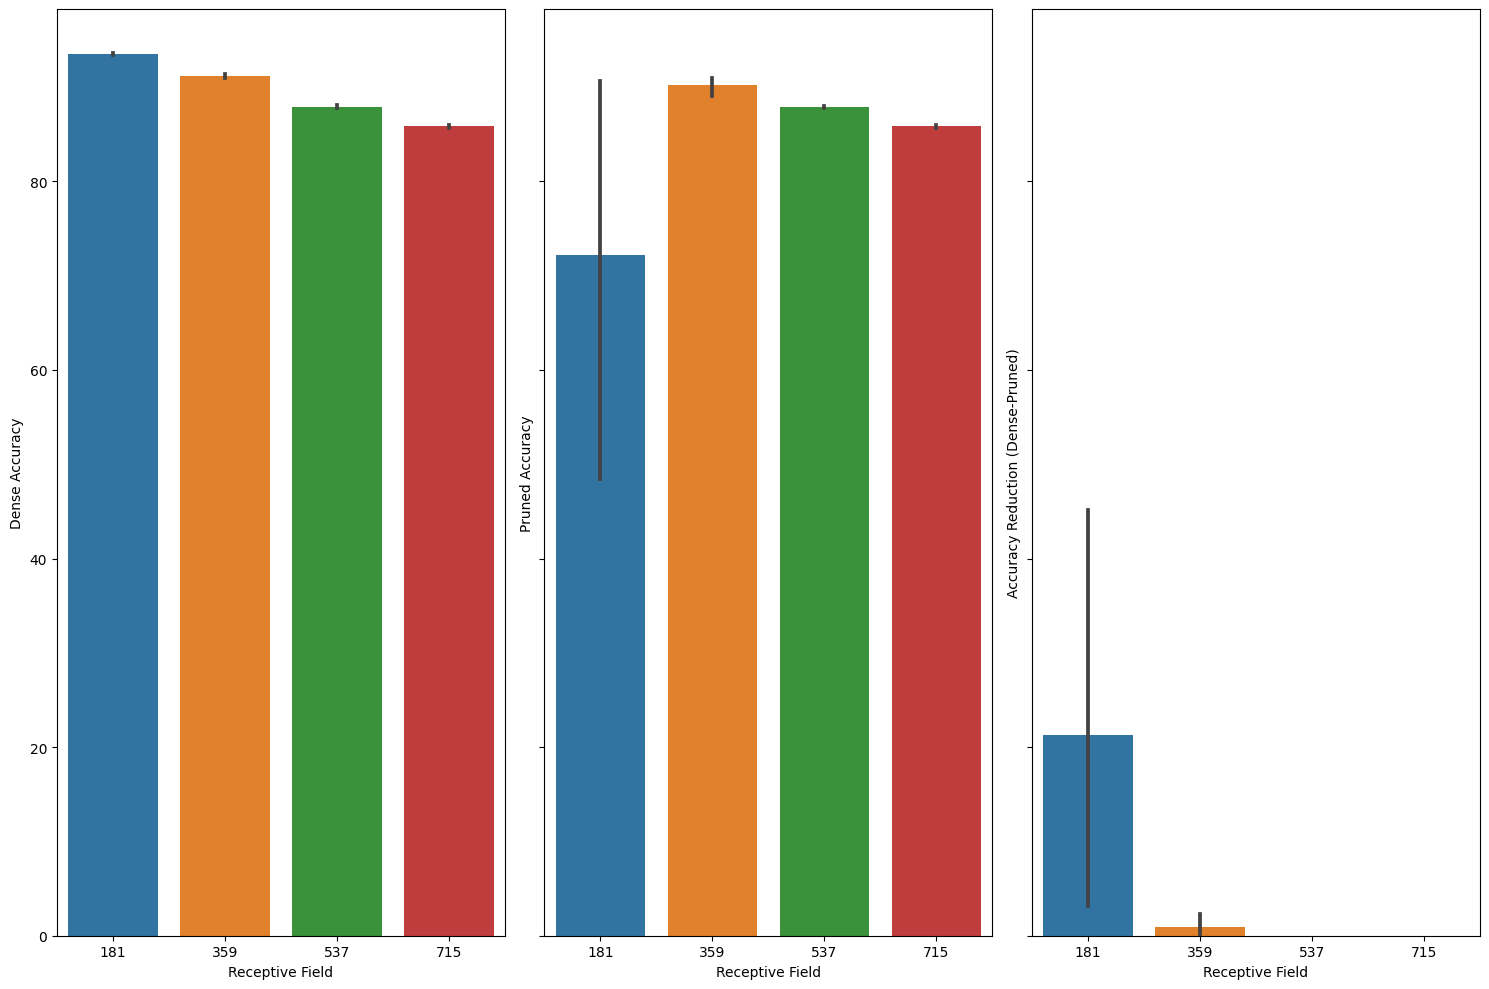
\includegraphics[width=1.1\columnwidth]{images/Supplementary_material/cifar10_vgg19_pruning_results_0.8.png}
    \caption{VGG}
    \label{subfig:vgg19CIfar10PR0.8}
     \end{subfigure}
      \hfill
     \begin{subfigure}[b]{\columnwidth}
    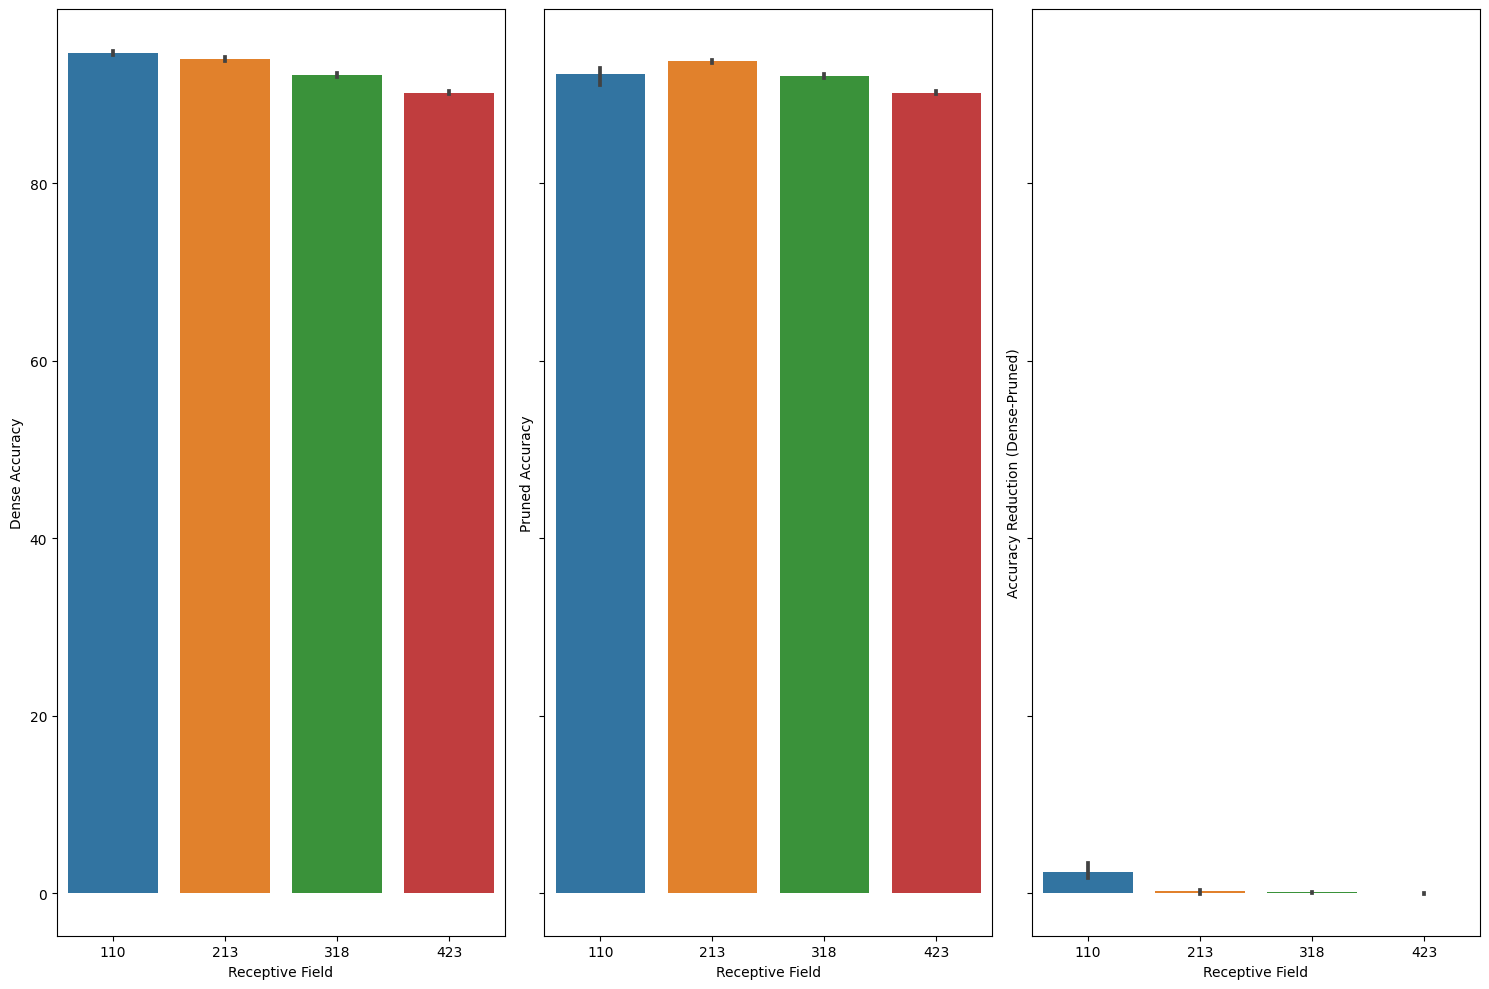
\includegraphics[width=1.1\columnwidth]{images/Supplementary_material/cifar10_resnet50_pruning_results_0.8.png}
    \caption{ResNet-50}
    \label{subfig:resenet50CIfar10PR0.8}
     \end{subfigure}
     \caption{ CIFAR10 pruning rate 0.8 results}
    \label{fig:pr_0.8_CIFAR10}
\end{figure}

\begin{figure}[h]
 \centering
     \begin{subfigure}[b]{\columnwidth}
    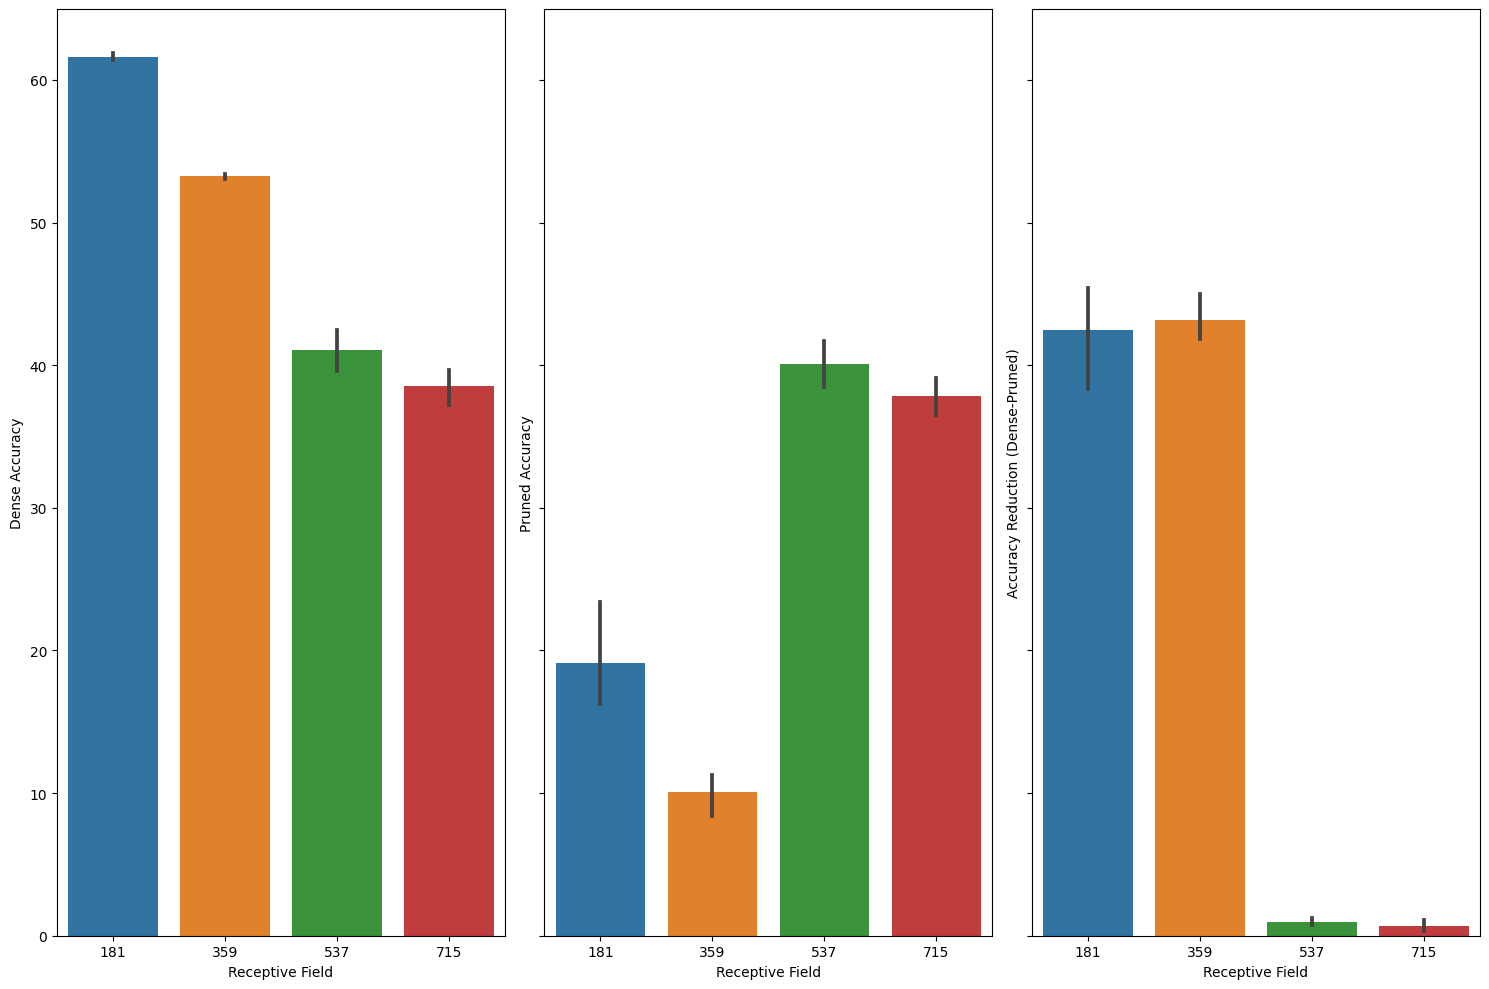
\includegraphics[width=1.1\columnwidth]{images/Supplementary_material/tiny_imagenet_vgg19_pruning_results_0.8.png}
    \caption{VGG}
    \label{subfig:vgg19CIfar10PR0.8}
     \end{subfigure}
      \hfill
     \begin{subfigure}[b]{\columnwidth}
    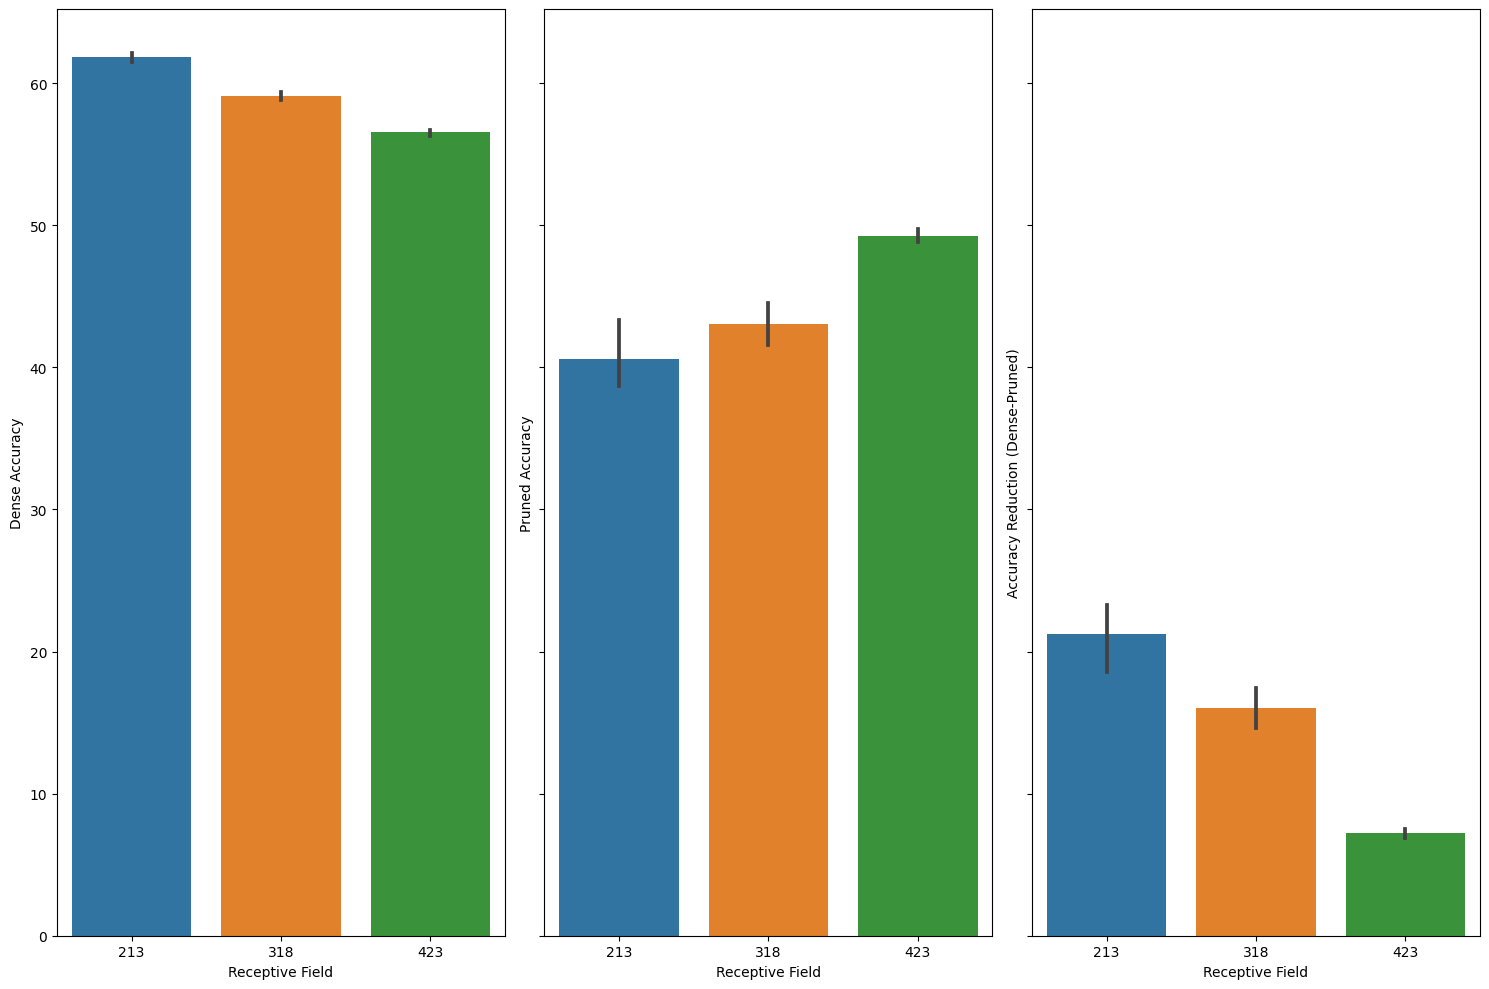
\includegraphics[width=1.1\columnwidth]{images/Supplementary_material/tiny_imagenet_resnet50_pruning_results_0.8.png}
    \caption{ResNet-50}
    \label{subfig:resenet50CIfar10PR0.8}
     \end{subfigure}
     \caption{ Tiny ImageNet pruning 0.8 results}
    \label{fig:pr_0.8_tiny_imagenet}
\end{figure}

\subsubsection*{Pruning rate 0.7}

\begin{figure}[h]
 \centering
     \begin{subfigure}[b]{\columnwidth}
    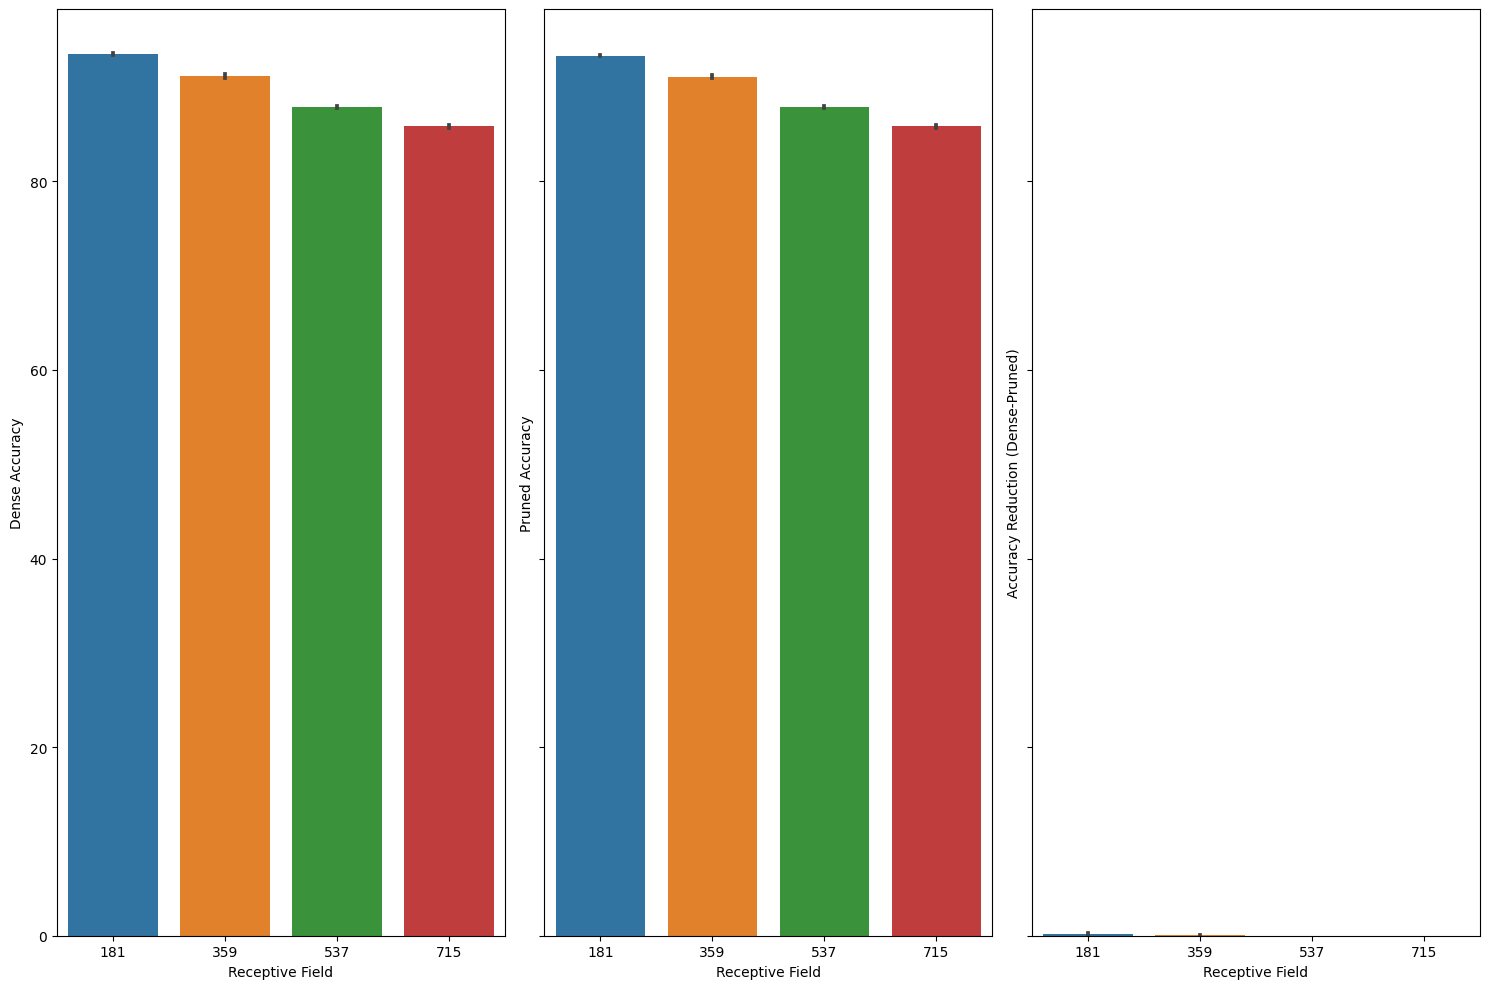
\includegraphics[width=1.1\columnwidth]{images/Supplementary_material/cifar10_vgg19_pruning_results_0.7.png}
    \caption{VGG}
    \label{subfig:vgg19CIfar10PR0.7}
     \end{subfigure}
      \hfill
     \begin{subfigure}[b]{\columnwidth}
    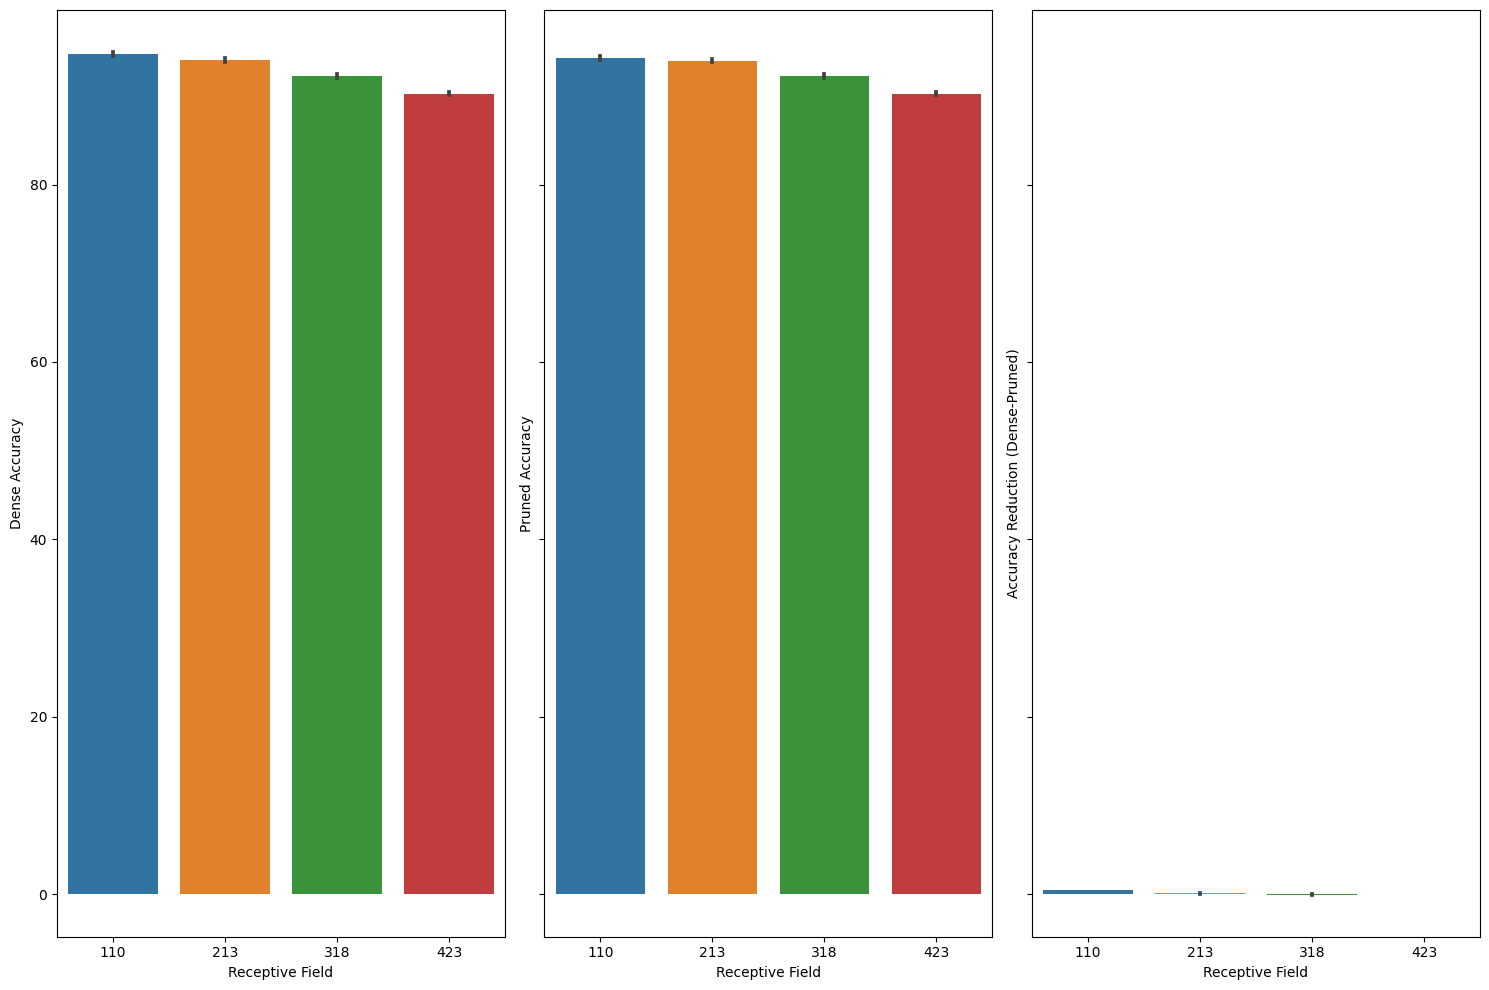
\includegraphics[width=1.1\columnwidth]{images/Supplementary_material/cifar10_resnet50_pruning_results_0.7.png}
    \caption{ResNet-50}
    \label{subfig:resenet50CIfar10PR0.7}
     \end{subfigure}
     \caption{ CIFAR10 0.7 results}
    \label{fig:pr_0.7_CIFAR10}
\end{figure}


\begin{figure}[h]
 \centering
     \begin{subfigure}[b]{\columnwidth}
    \includegraphics[width=1.1\columnwidth]{images/Supplementary_material/tiny_imagenet_vgg19_pruning_results_0.7.png}
    \caption{VGG}
    \label{subfig:vgg19CIfar10PR0.7}
     \end{subfigure}
      \hfill
     \begin{subfigure}[b]{\columnwidth}
    \includegraphics[width=1.1\columnwidth]{images/Supplementary_material/tiny_imagenet_resnet50_pruning_results_0.7.png}
    \caption{ResNet-50}
    \label{subfig:resenet50CIfar10PR0.7}
     \end{subfigure}
     \caption{ Tiny ImageNet pruning 0.7 results}
    \label{fig:pr_0.7_tiny_imagenet}
\end{figure}

\subsubsection*{Pruning rate 0.6}

\begin{figure}[h]
 \centering
     \begin{subfigure}[b]{\columnwidth}
    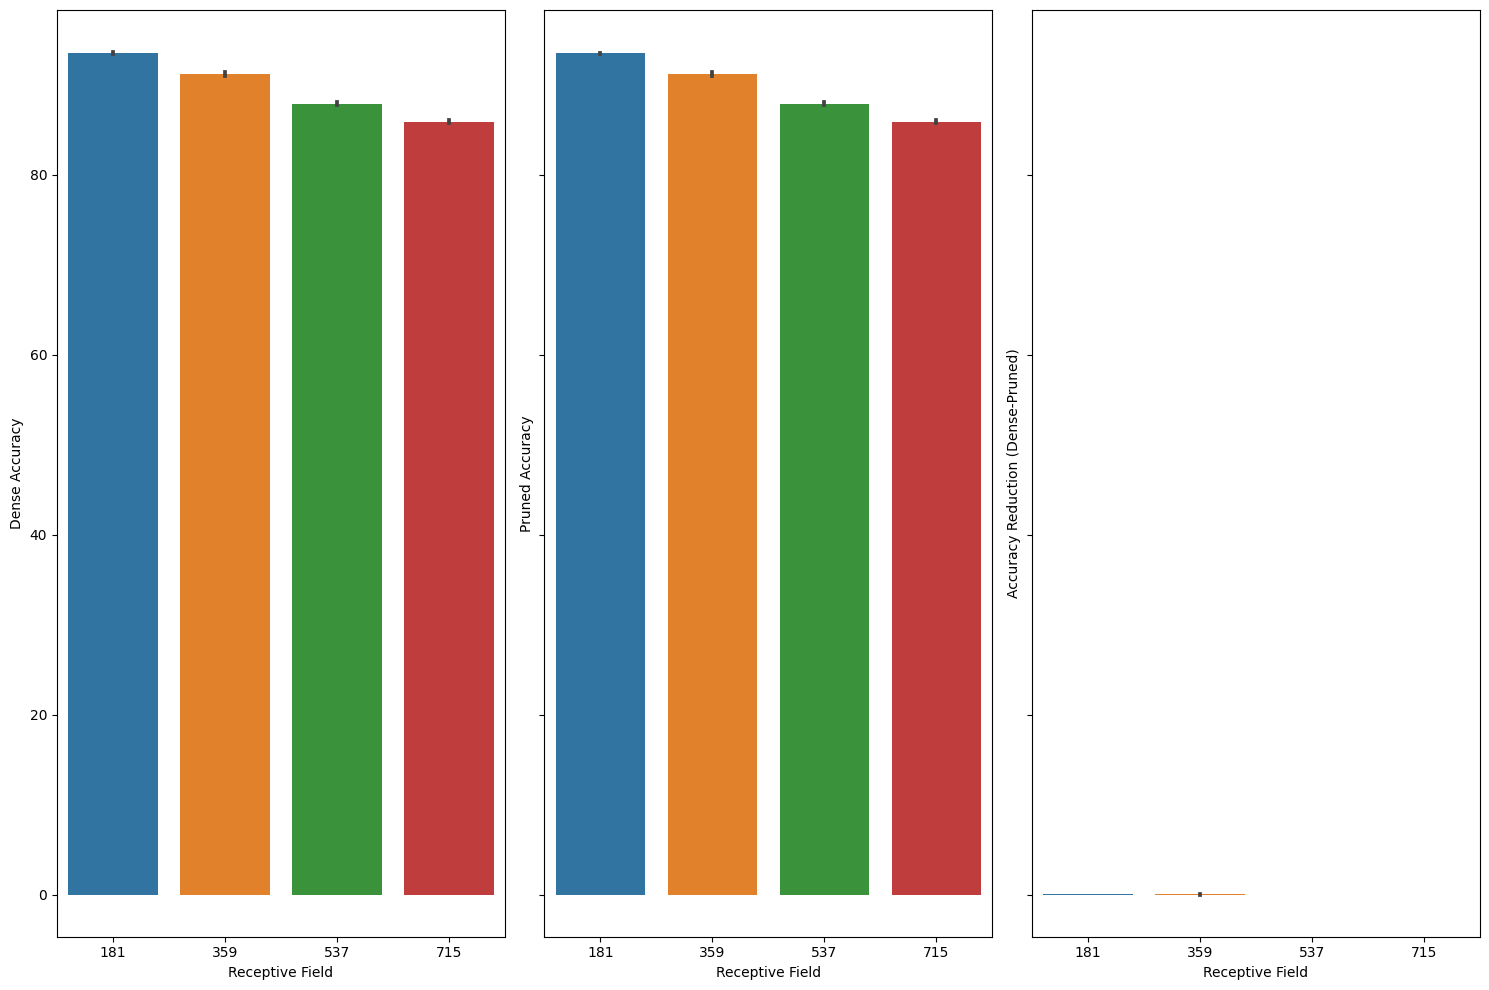
\includegraphics[width=1.1\columnwidth]{images/Supplementary_material/cifar10_vgg19_pruning_results_0.6.png}
    \caption{VGG}
    \label{subfig:vgg19CIfar10PR0.6}
     \end{subfigure}
      \hfill
     \begin{subfigure}[b]{\columnwidth}
    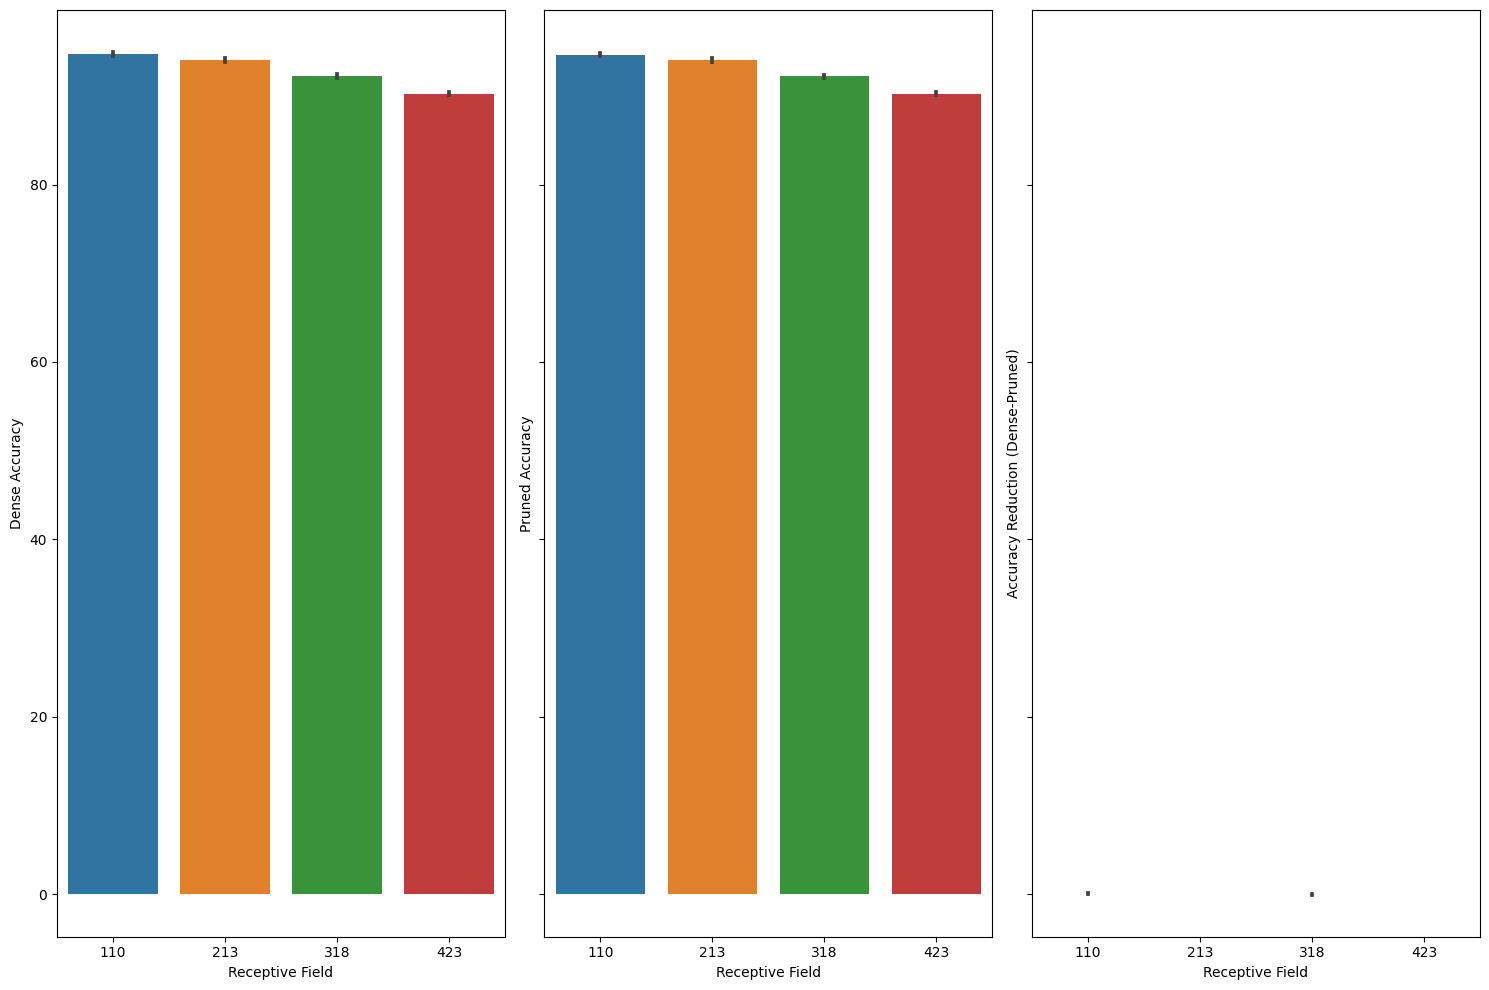
\includegraphics[width=1.1\columnwidth]{images/Supplementary_material/cifar10_resnet50_pruning_results_0.6.png}
    \caption{ResNet-50}
    \label{subfig:resenet50CIfar10PR0.6}
     \end{subfigure}
     \caption{ CIFAR10 0.6 results}
    \label{fig:pr_0.7_CIFAR10}
\end{figure}


\begin{figure}[h]
 \centering
     \begin{subfigure}[b]{\columnwidth}
    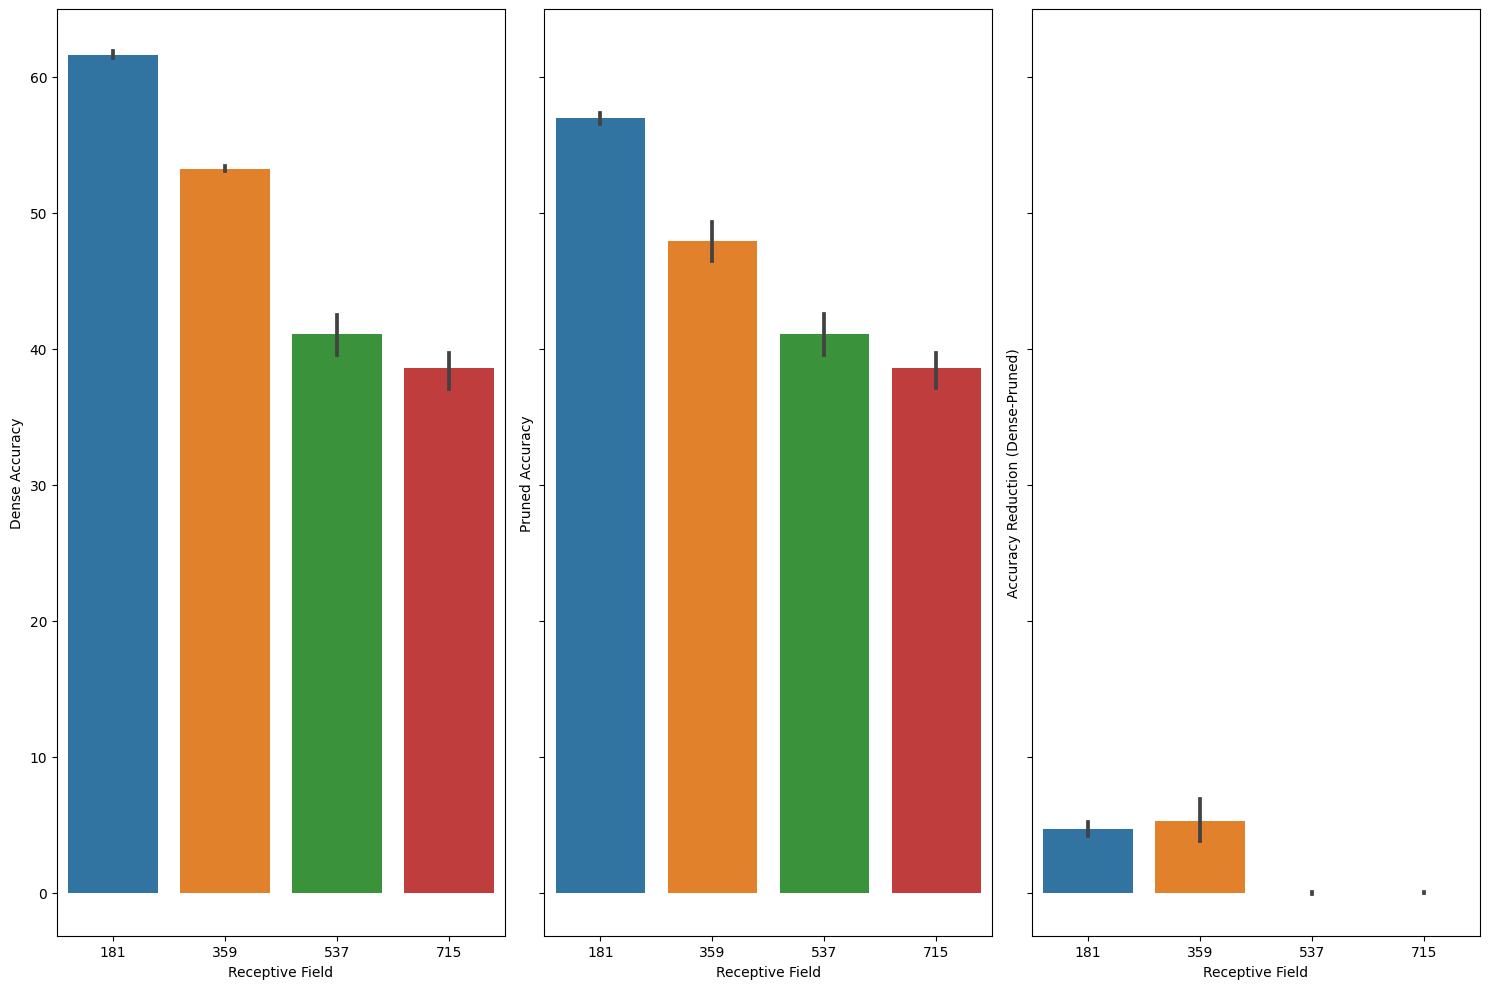
\includegraphics[width=1.1\columnwidth]{images/Supplementary_material/tiny_imagenet_vgg19_pruning_results_0.6.png}
    \caption{VGG}
    \label{subfig:vgg19CIfar10PR0.6}
     \end{subfigure}
      \hfill
     \begin{subfigure}[b]{\columnwidth}
    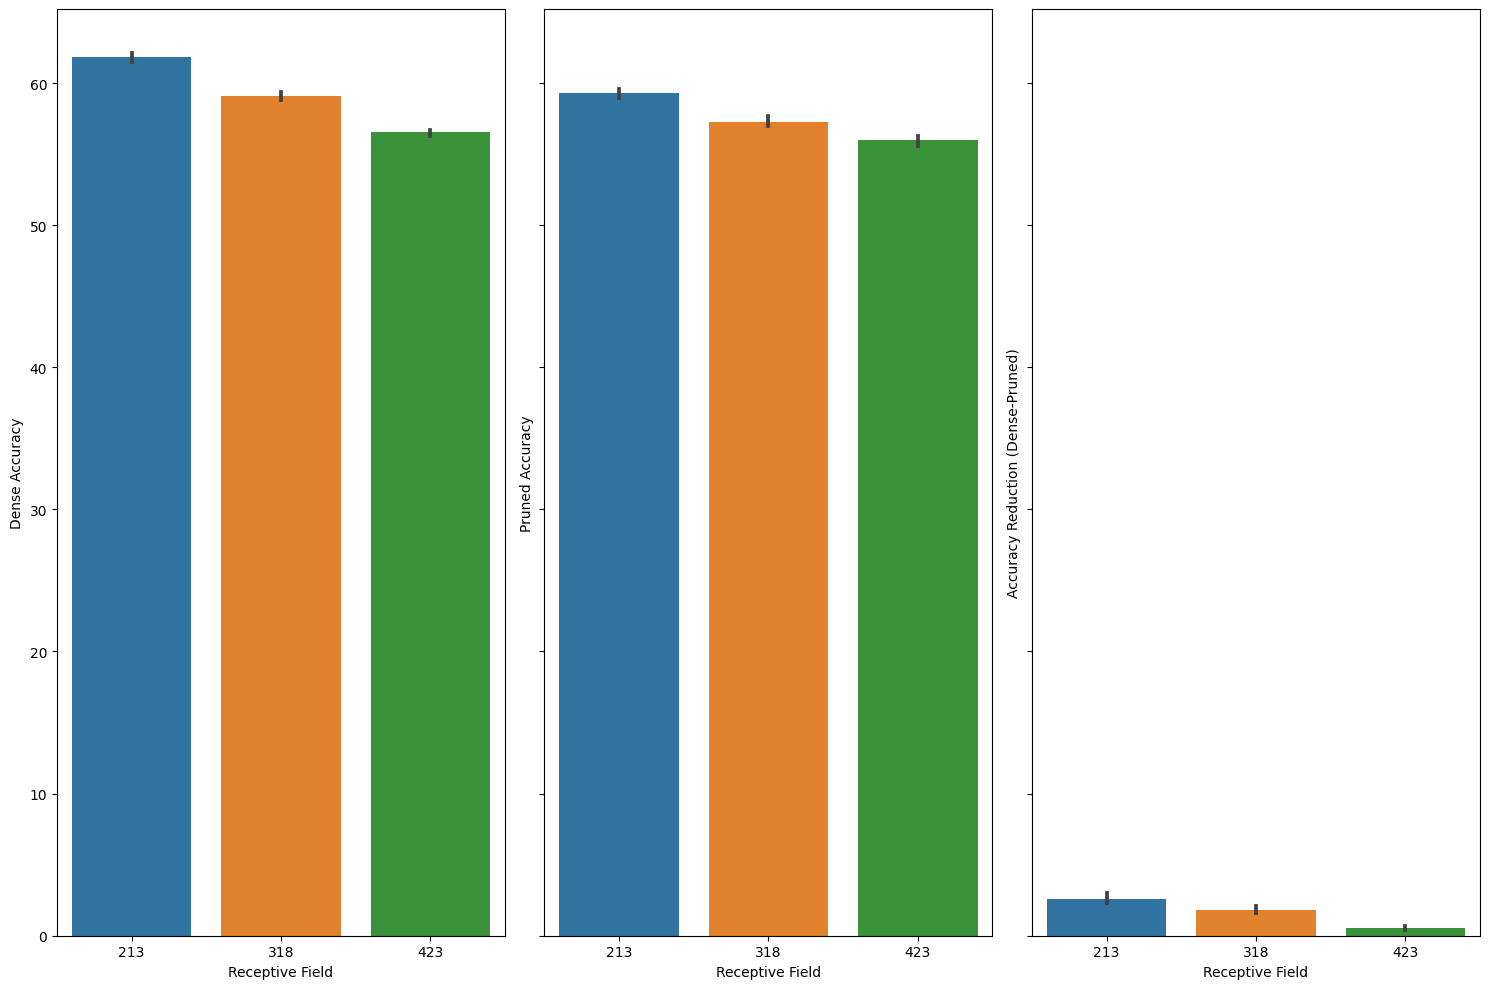
\includegraphics[width=1.1\columnwidth]{images/Supplementary_material/tiny_imagenet_resnet50_pruning_results_0.6.png}
    \caption{ResNet-50}
    \label{subfig:resenet50CIfar10PR0.6}
     \end{subfigure}
     \caption{ Tiny ImageNet 0.6 results}

    \label{fig:pr_0.6_tiny_imagenet}

\end{figure}

\subsubsection*{Pruning rate 0.5}

\begin{figure}[h]
 \centering
     \begin{subfigure}[b]{\columnwidth}
    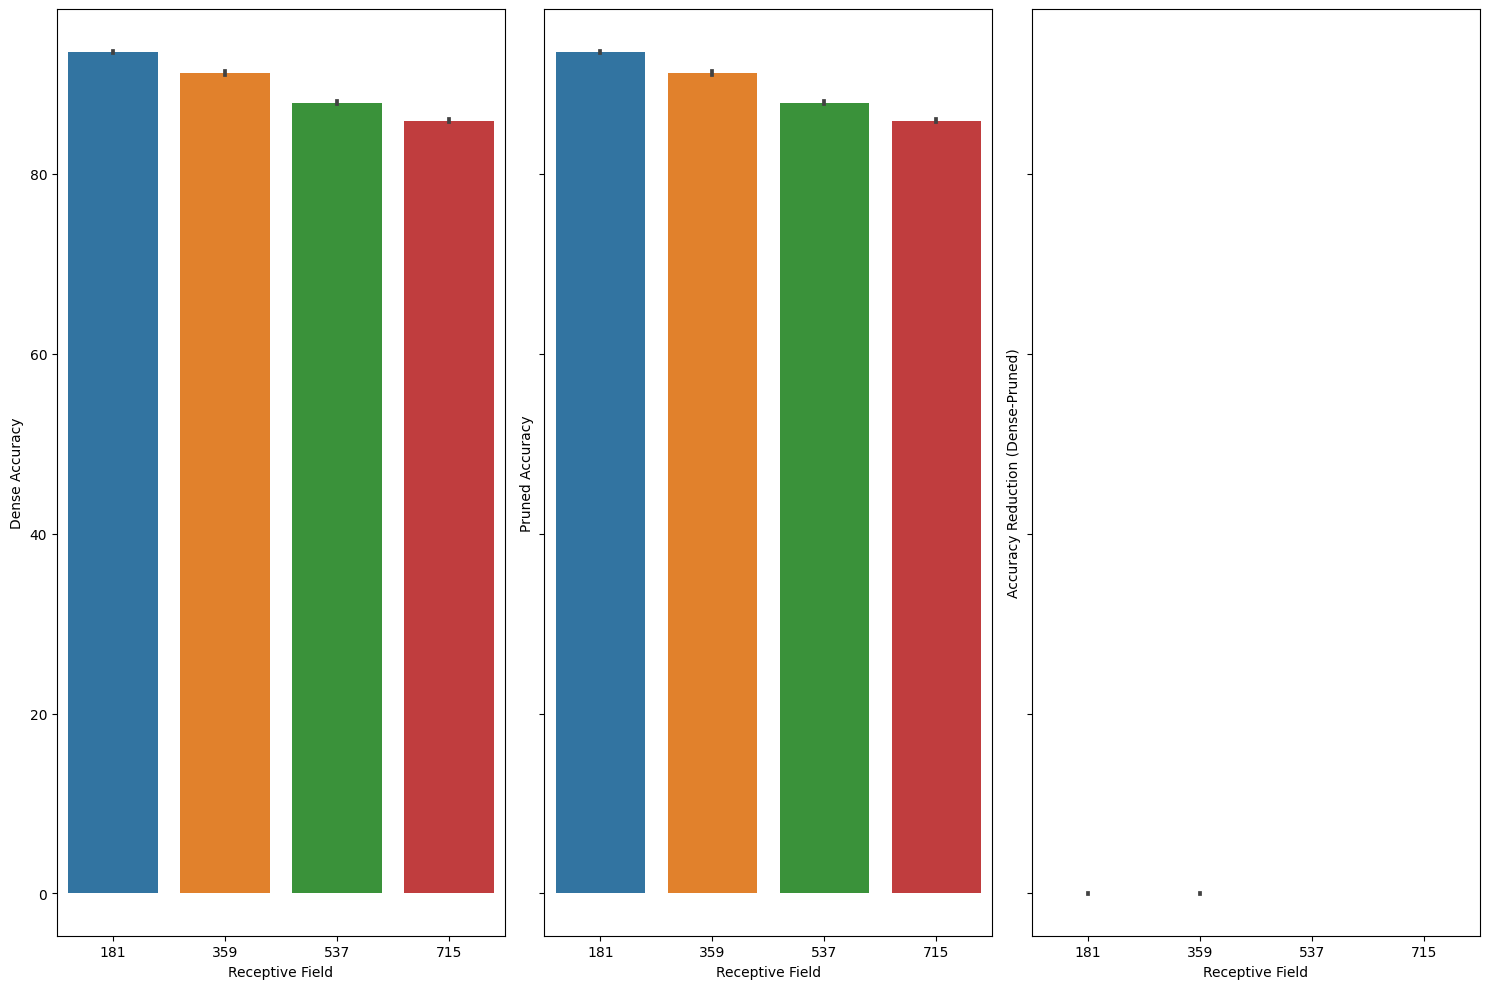
\includegraphics[width=1.1\columnwidth]{images/Supplementary_material/cifar10_vgg19_pruning_results_0.5.png}
    \caption{VGG}
    \label{subfig:vgg19CIfar10PR0.5}
     \end{subfigure}
      \hfill
     \begin{subfigure}[b]{\columnwidth}
    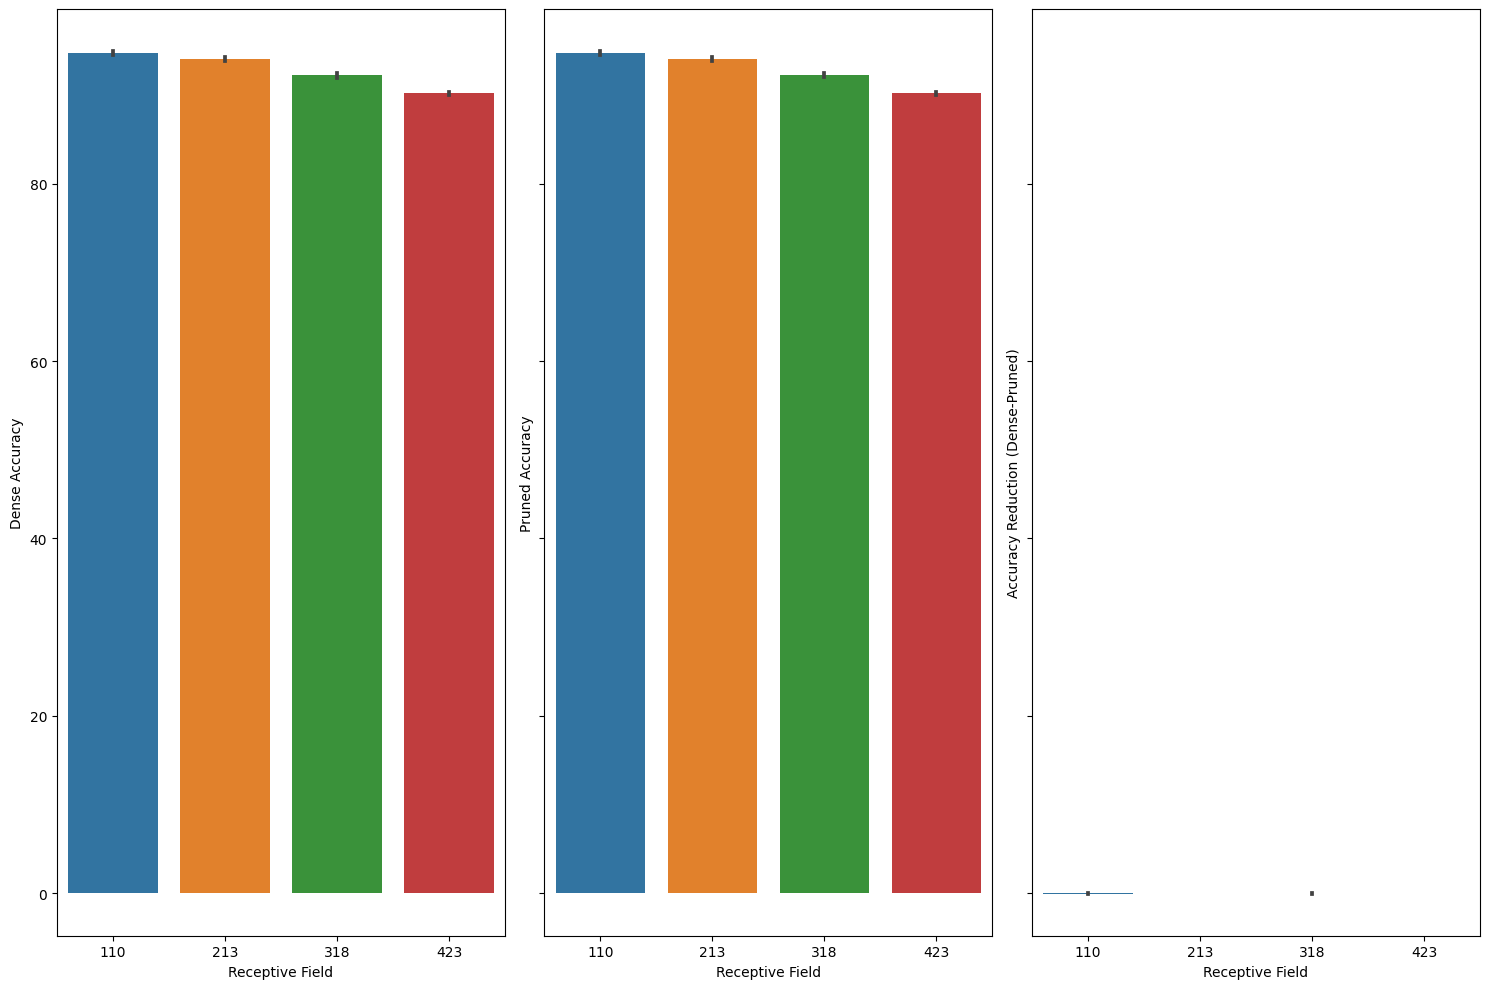
\includegraphics[width=1.1\columnwidth]{images/Supplementary_material/cifar10_resnet50_pruning_results_0.5.png}
    \caption{ResNet-50}
    \label{subfig:resenet50CIfar10PR0.5}
     \end{subfigure}
     \caption{ CIFAR10 0.5 results}
    \label{fig:pr_0.5_CIFAR10}
\end{figure}


\begin{figure}[h]
 \centering
     \begin{subfigure}[b]{\columnwidth}
    \includegraphics[width=1.1\columnwidth]{images/Supplementary_material/tiny_imagenet_vgg19_pruning_results_0.5.png}
    \caption{VGG}
    \label{subfig:vgg19CIfar10PR0.5}
     \end{subfigure}
      \hfill
     \begin{subfigure}[b]{\columnwidth}
    \includegraphics[width=1.1\columnwidth]{images/Supplementary_material/tiny_imagenet_resnet50_pruning_results_0.5.png}
    \caption{ResNet-50}
    \label{subfig:resenet50CIfar10PR0.5}
     \end{subfigure}
     \caption{ Tiny ImageNet pruning 0.5 results}
    \label{fig:pr_0.8_tiny_imagenet}
\end{figure}



\subsection*{Fine-tuning pruned solutions}
\label{subsec:Fine_tuning_solutions}
Here we fine-tuned the pruned solutions while preserving the mask for 10 epochs with the following hyper-parameters
\begin{itemize}
  \item Initial Learning Rate: 0.0001,
  \item Weight Decay:5e-4
  \item Momentum:0,9
  \item Gradient clip: 0.1
\end{itemize}

\todo[inline]{All of the following figures would be better on a table}
\begin{figure}[!htb]
 \centering
     \begin{subfigure}[b]{\columnwidth}
    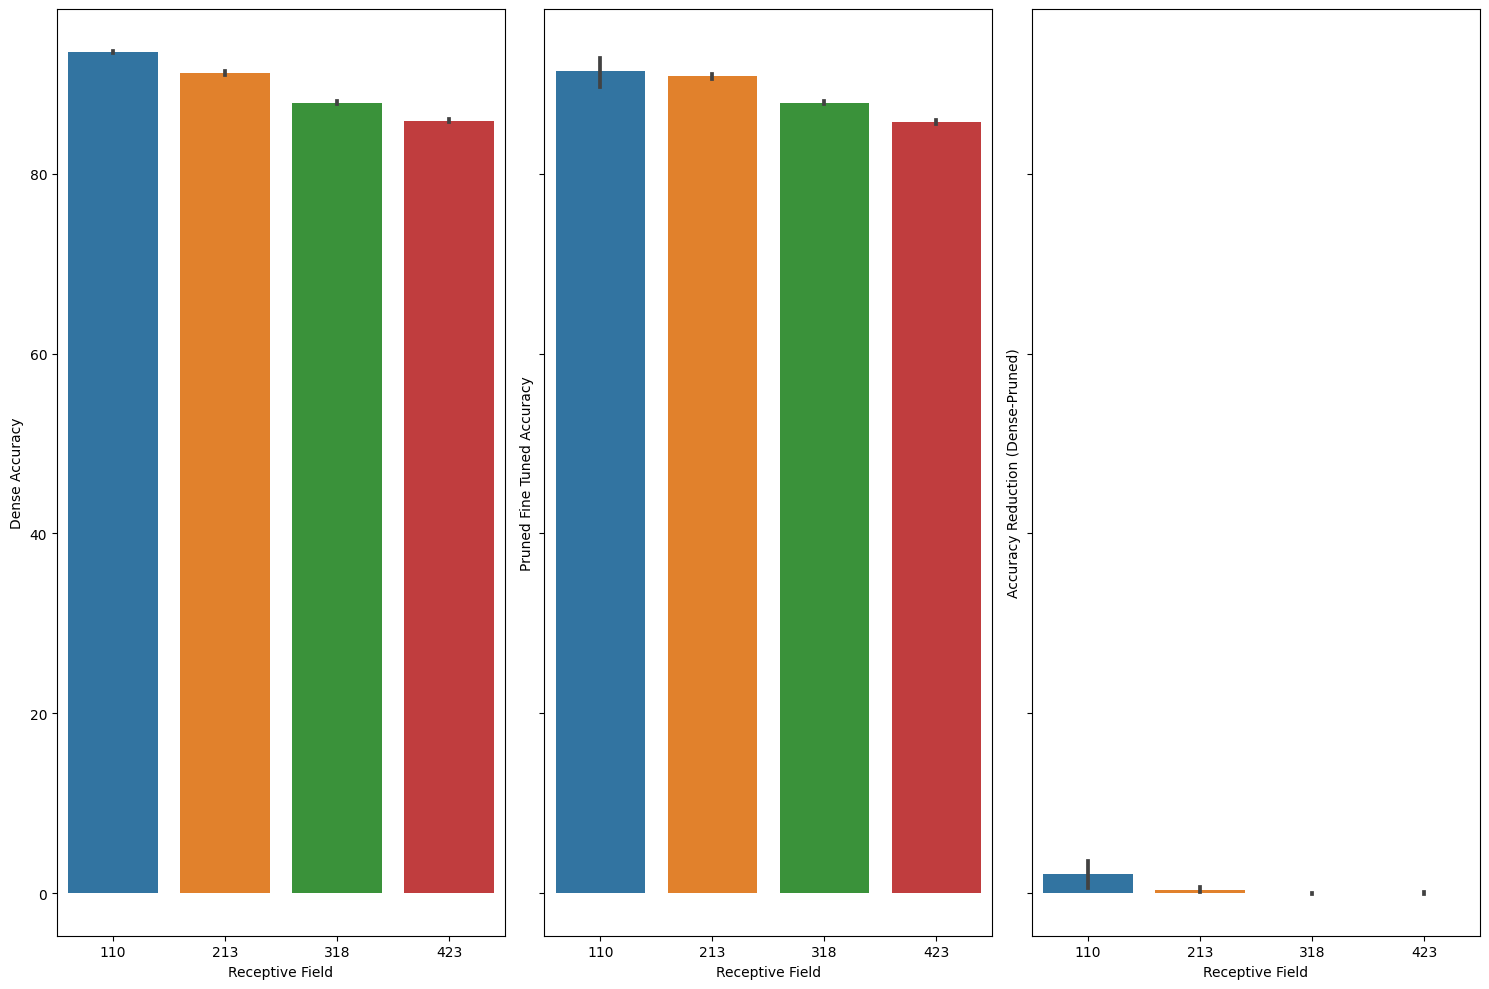
\includegraphics[width=1.1\columnwidth]{images/Supplementary_material/cifar10_vgg19_pruning_finetuned_results_0.9.png}
    \caption{VGG}
    \label{subfig:vgg19CIfar10FInetuned}
     \end{subfigure}
      \hfill
     \begin{subfigure}[b]{\columnwidth}
    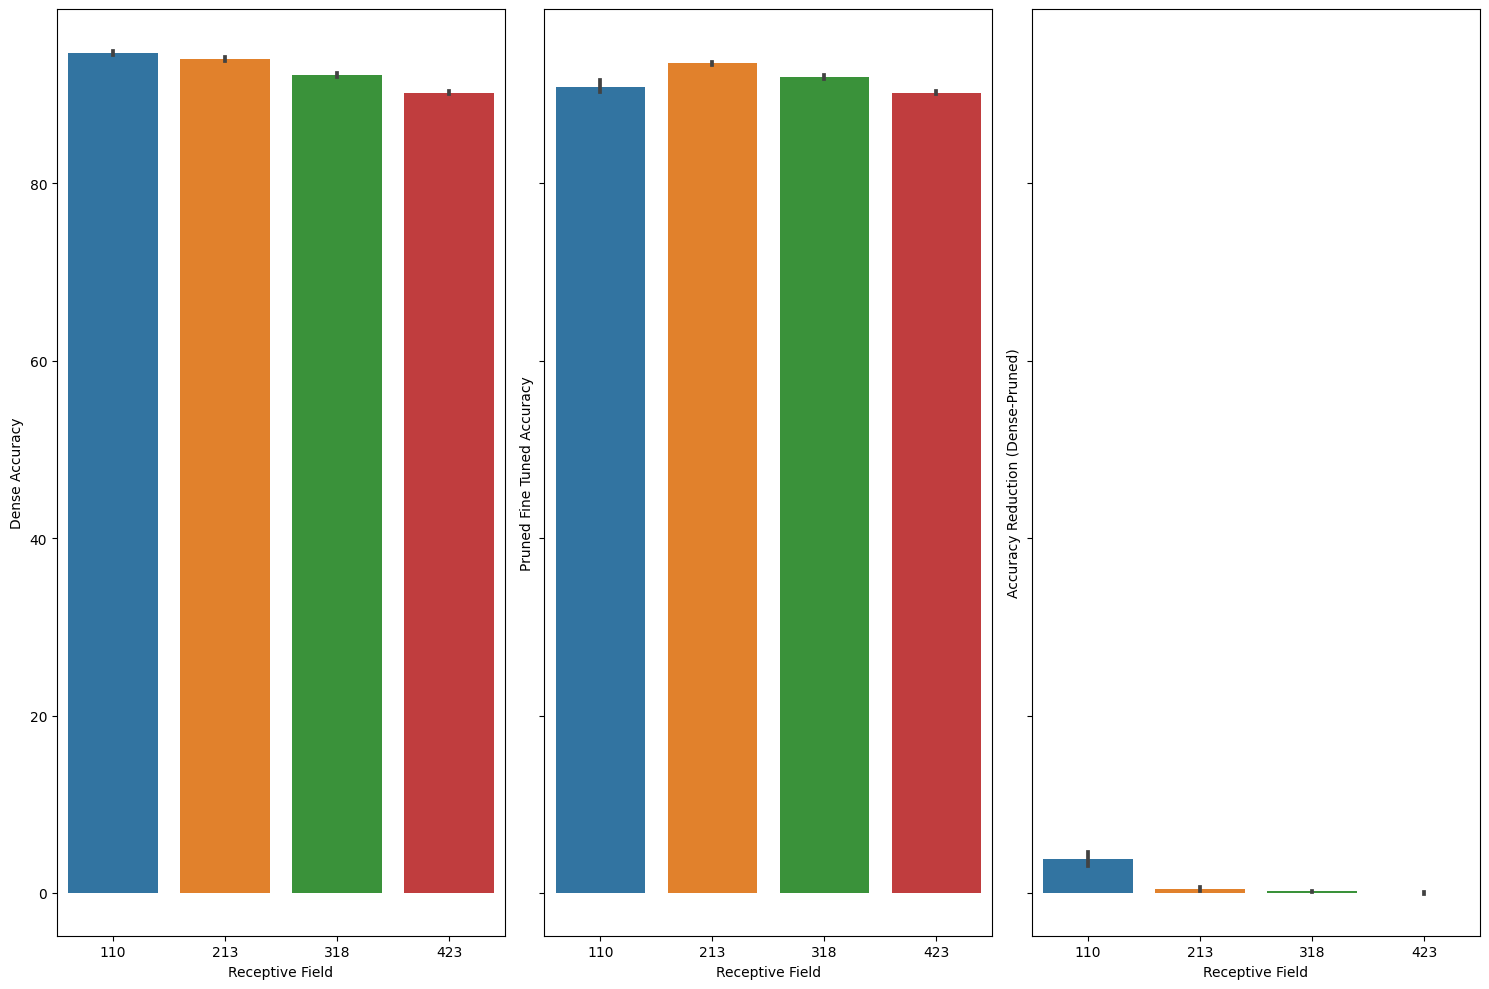
\includegraphics[width=1.1\columnwidth]{images/Supplementary_material/cifar10_resnet50_pruning_finetuned_results_0.9.png}
    \caption{ResNet-50}
    \label{subfig:resenet50CIfar10FInetuned}
     \end{subfigure}
     \caption{ CIFAR10 Fine-tuned results}
    \label{fig:finetuned_CIFAR10}
  \end{figure}

\begin{figure*}[!htb]
 \centering
     \begin{subfigure}[b]{\columnwidth}
    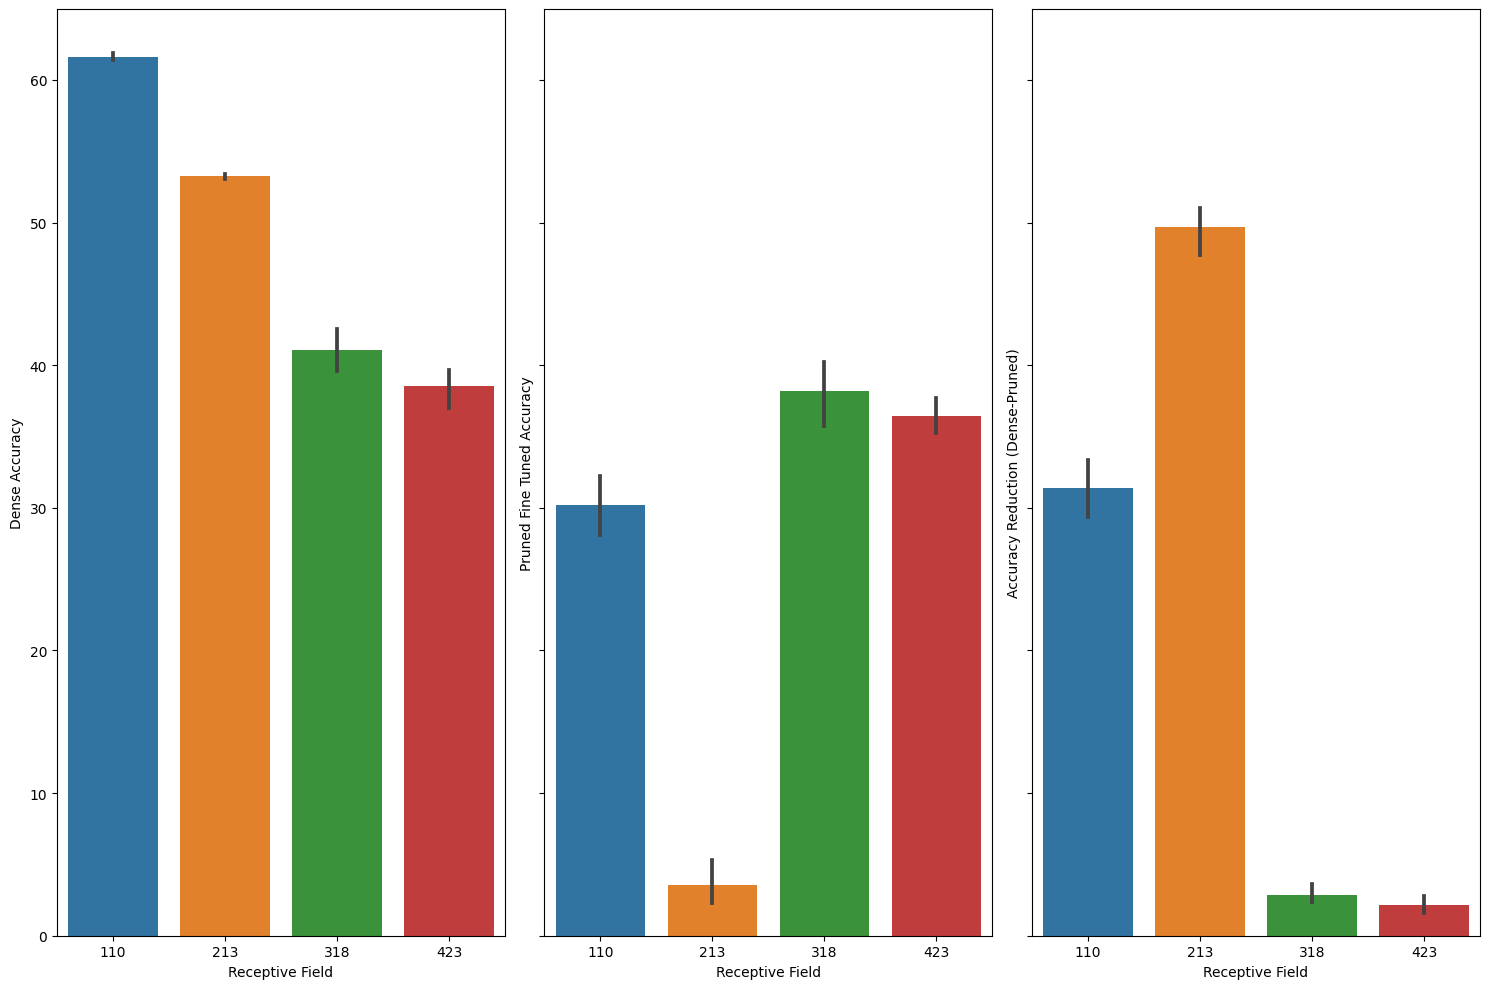
\includegraphics[width=1.1\columnwidth]{images/Supplementary_material/tiny_imagenet_vgg19_pruning_finetuned_results_0.9.png}
    \caption{VGG}
    \label{subfig:vgg19_tiny_imagenet_FInetuned}
     \end{subfigure}
      \hfill
     \begin{subfigure}[b]{\columnwidth}
    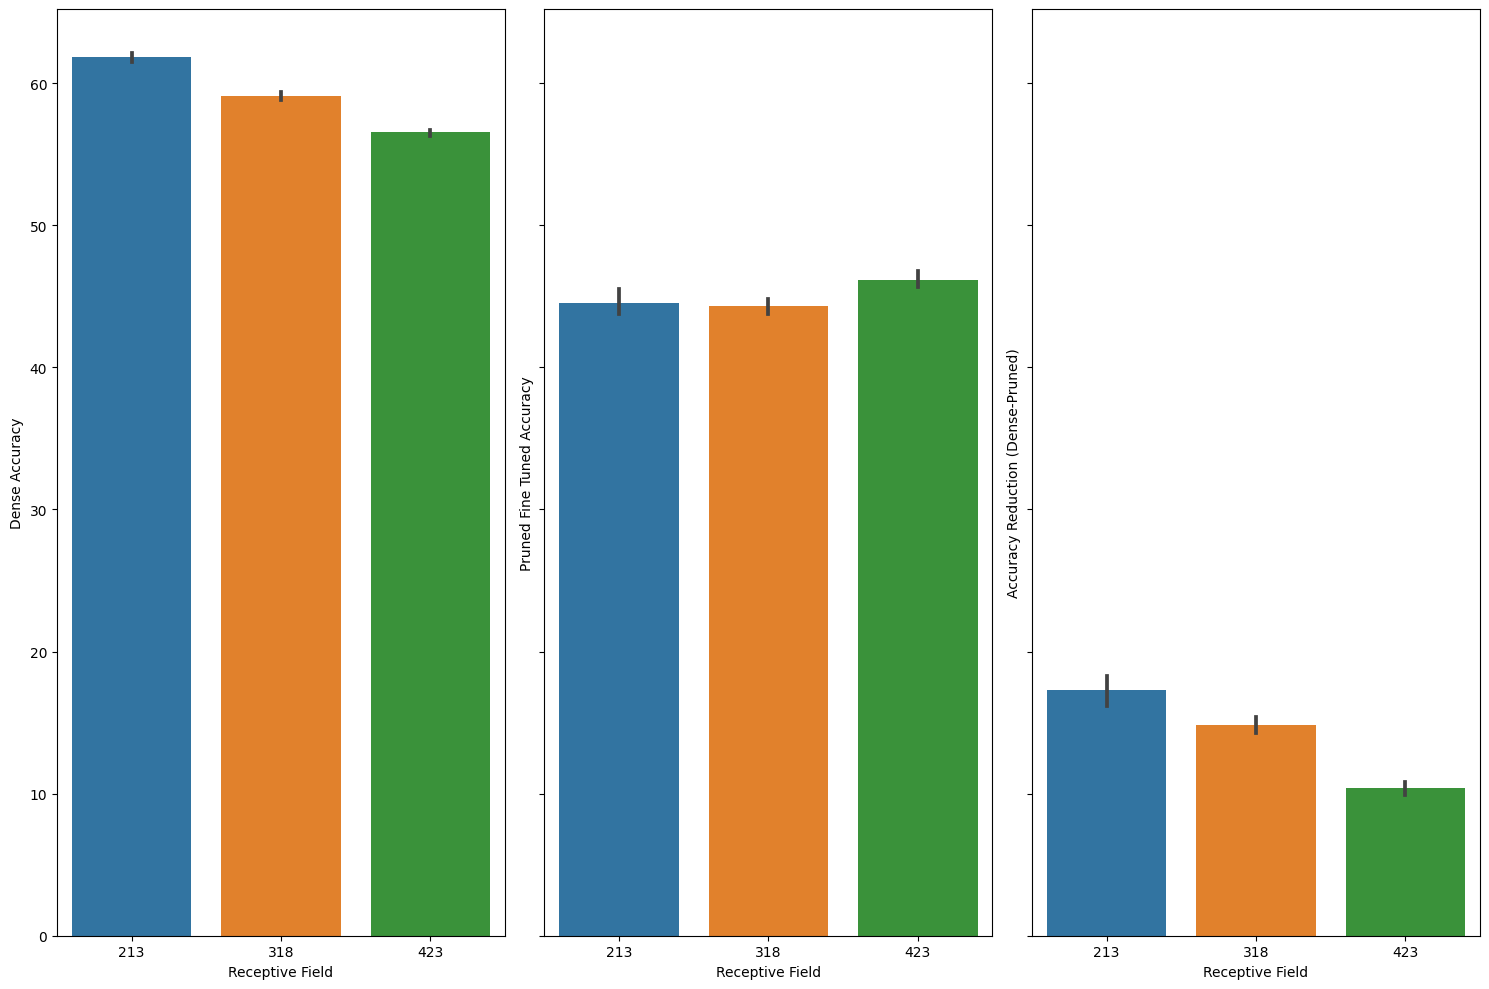
\includegraphics[width=1.1\columnwidth]{images/Supplementary_material/tiny_imagenet_resnet50_pruning_finetuned_results_0.9.png}
    \caption{ResNet-50}
    \label{subfig:resenet50tiny_imagenetFinetuned}
     \end{subfigure}
     \caption{Tiny ImageNet Fine-tuned results}
    \label{fig:finetuned_tiny_imagenet}
\end{figure*}
